\documentclass[a4paper, 24pt]{article}
% Page Margins
\usepackage[margin=1in]{geometry}
\usepackage{graphicx}
\usepackage{subcaption}

% Font Specification
\usepackage{fontspec}
\setmainfont{JetBrainsMono-Medium}[
Extension = .ttf,
]
\usepackage{float}
% AMS Packages
\usepackage{amsmath, amsthm, amssymb}
\usepackage{titlesec}
\usepackage{color}
\definecolor{sectioncolor}{RGB}{0,0,139} % Navy Blue
\definecolor{subsectioncolor}{RGB}{0,100,0} % Dark Green
\definecolor{subsubsectioncolor}{RGB}{139,0,0} % Dark Red

% Unicode and Hyperlinks
\usepackage[utf8]{inputenc}
\usepackage{hyperref}
\hypersetup{
unicode,
pdfauthor={Sri Ganesh Thota},
pdftitle={PRML Project Report},
pdfsubject={PRML Project Report},
pdfkeywords={music recommendation, PRML, project report},
pdfproducer={LaTeX},
pdfcreator={pdflatex}
}

% Bibliography Style
\usepackage[sort&compress,numbers,square]{natbib}
\bibliographystyle{mplainnat}

% Graphics
\usepackage{graphicx, color}
\graphicspath{{fig/}}

% Algorithms
\usepackage{algorithm, algpseudocode}

% Mathematical Script
\usepackage{mathrsfs}

% Dummy Text
\usepackage{lipsum}

% Font Size Adjustments
\renewcommand{\normalsize}{\fontsize{14}{16}\selectfont} % Body + 2
\newcommand{\abstractfont}{\fontsize{12}{14}\selectfont} % Abstract - 2
\title{\fontsize{16}{18}\selectfont Music Classifier and Recommendation System} % Title + 2
\titleformat{\section}
{\color{sectioncolor}\normalfont\Large\bfseries}
{\color{sectioncolor}\thesection}{1em}{}

\titleformat{\subsection}
{\color{subsectioncolor}\normalfont\large\bfseries}
{\color{subsectioncolor}\thesubsection}{1em}{}

\titleformat{\subsubsection}
{\color{subsubsectioncolor}\normalfont\normalsize\bfseries}
{\color{subsubsectioncolor}\thesubsubsection}{1em}{}
\titlespacing*{\section}{0pt}{3.5ex plus 1ex minus .2ex}{2.3ex plus .2ex}
\titlespacing*{\subsection}{0pt}{3.25ex plus 1ex minus .2ex}{1.5ex plus .2ex}
\titlespacing*{\subsubsection}{0pt}{3.25ex plus 1ex minus .2ex}{1.5ex plus .2ex}

% Author Info
\author{
Sri Ganesh Thota$^1$ \and
Rahul Reddy Purmani$^2$ \and
Karan Reddy Kanakanala$^3$ \and
Abhijan Theja Katukojwala $^4$ \and
Aditya Trivedi Bhargavkumar $^5$ \and
Shubham Kumar $^6$ \and
Kaushik Salla $^7$
}

\date{
Indian Institute of Technology Jodhpur \\ 
\texttt{\{b22cs054, b22cs041, b22ai023, b22ai025, b22cs055, b22ee064, b22ee058\}@iitj.ac.in} \\
\texttt{Submitted to Prof. Anand Mishra} \\ 
\today
}
\begin{document}

\maketitle

\begin{abstract}
\abstractfont
The digital music landscape is vast, offering listeners a plethora of choices. This vastness can be overwhelming, making efficient music discovery challenging. This project addresses this by developing a personalized music recommendation system based solely on song names and a robust music genre classification system.

Our personalized music recommendation system uses machine-learning techniques to generate song suggestions based on song names. While it doesn't delve into user listening history or preferences, it provides a convenient way for users to discover new songs that align with their current interests. The system's simplicity and efficiency make it a valuable tool for quick and easy music exploration.

In contrast, our music genre classification system employs various machine learning algorithms such as Logistic Regression, SVM, Random Forest, and Light GBM. We rigorously evaluate these algorithms using real-world datasets, demonstrating their effectiveness in accurately classifying songs into distinct genres.

Through comprehensive evaluation and user studies, we showcase the strengths of both systems. The recommendation system simplifies song discovery, while the classification system offers a structured approach to exploring music genres. Together, these systems aim to enhance user engagement and navigation within the digital music landscape.
\end{abstract}

\newpage

\tableofcontents

\newpage

\section{Introduction}
\label{sec:intro}

Greetings,

In the era of digital music streaming, listeners are presented with an overwhelming variety of song choices. This wealth of options, while a testament to the diversity of musical content available, poses a challenge: how can listeners efficiently discover new songs that align with their current interests? This project introduces two distinct systems to address this challenge: a personalized music recommendation system and a music genre classification system.

\subsection{Problem Statement}

The digital music landscape offers a vast array of songs and artists. However, users often struggle to efficiently discover new music that resonates with their tastes. The primary issue is the difficulty in navigating this vast library to find songs of interest.

The two-fold problem addressed by this project includes:

\begin{itemize}
\item Personalized Music Recommendation System: To simplify song discovery, we've developed a recommendation system that suggests songs based solely on song names. While it doesn't take into account user listening history or preferences, it offers a straightforward way for users to explore new songs.
\item Music Genre Classification System: Understanding the importance of music genres in guiding song discovery, we've implemented a classification system that categorizes songs into distinct genres. Leveraging machine learning algorithms like Logistic Regression, SVM, Random Forest, and Light GBM, this system provides a structured approach to exploring music by genre.
\end{itemize}

Our project aims to:

\begin{itemize}
\item Enhance the song discovery process by providing a simple and efficient personalized music recommendation system based on song names.
\item Facilitate genre-based music exploration through a robust music genre classification system, aiding users in discovering songs within their preferred genres.
\item Improve user engagement and satisfaction by offering diverse yet relevant song suggestions and structured genre classifications, enhancing the overall music streaming experience.
\end{itemize}

Through implementing and evaluating these two systems, we aspire to revolutionize how listeners interact with and discover music on streaming platforms, catering to both the casual listener and the genre enthusiast.

\subsection{Report Structure}

The structure of this report has been meticulously designed to provide a comprehensive insight into our project's development, methodology, and findings. It is organized as follows:

\begin{itemize}
\item \textbf{Section 2: Approaches Tried} - 
This section delves into various machine learning algorithms we explored. We discuss the rationale behind each choice, the methodologies employed, and the challenges faced. We also provide a detailed comparison highlighting strengths and weaknesses.

\item \textbf{Section 3: Experiments and Results} - 
Here, we describe experiments conducted to evaluate algorithm performance. We discuss the dataset, experimental settings, and evaluation metrics used. A comprehensive analysis of results showcases algorithm effectiveness.

\item \textbf{Section 4: Summary} - 
This section culminates our project, summarizing key findings and contributions. We reflect on the system's performance, potential industry impact, and future research areas. 

\item \textbf{Appendix A: Contribution of Each Member} - 
In this appendix, we detail contributions by each team member. This includes roles undertaken, tasks completed, and unique insights contributed. 
\end{itemize}


We believe our structured approach will enable readers to navigate through the report seamlessly, gaining a thorough understanding of our system's development, evaluation, and implications. Delve into the following sections to explore our journey in designing this innovative system.


\section{Approaches Tried}
\label{sec:app}
In our pursuit of designing an effective personalized music recommendation system, we explored various machine learning algorithms. Each algorithm was fine-tuned using grid search to identify the optimal hyperparameters for maximizing accuracy. Below, we provide brief notes on the different approaches we tried:
\subsection{Classifier}
\subsubsection{Logistic Regression}
Logistic Regression is a linear model primarily used for binary classification problems. It models the probability that the target variable belongs to a particular category. We employed the LogisticRegression class from scikit-learn with regularization.

\subsubsection{SGD Classifier}
Stochastic Gradient Descent (SGD) Classifier is an optimization algorithm that updates the model's weights iteratively. The SGD Classifier in scikit-learn supports various loss functions and penalties for classification.

\subsubsection{Support Vector Machine (SVM)}
Support Vector Machine is a versatile supervised learning algorithm used for classification and regression tasks. It works by finding the hyperplane that best separates the data points into different classes. We utilized the SVC class from scikit-learn for our experiments.

\subsubsection{Random Forest}
Random Forest is an ensemble learning method that constructs multiple decision trees during training and outputs the class that is the mode of the classes (classification) of the individual trees. It combines their predictions through averaging or voting. We employed the RandomForestClassifier from scikit-learn.

\subsubsection{Decision Tree}
Decision Tree is a tree-like model used for both classification and regression. It breaks down a dataset into smaller subsets while recursively building a decision tree based on the features. We utilized the DecisionTreeClassifier from scikit-learn for our experiments.

\subsubsection{AdaBoost}
AdaBoost, short for Adaptive Boosting, is an ensemble learning method that combines multiple weak classifiers to create a strong classifier. It focuses more on the misclassified instances by assigning them higher weights. We employed the AdaBoostClassifier from scikit-learn.

\subsubsection{XGBoost}
XGBoost stands for Extreme Gradient Boosting, an optimized distributed gradient boosting library. It is highly efficient, flexible, and portable. XGBoost is an extension of the gradient boosting framework that includes regularization. We utilized the XGBClassifier from the XGBoost library.

\subsubsection{Gaussian Naive Bayes}
Gaussian Naive Bayes is a simple probabilistic classifier based on applying Bayes' theorem with strong (naive) independence assumptions between features. It assumes that the presence (or absence) of a particular feature of a class is unrelated to the presence (or absence) of any other feature. We employed the GaussianNB class from scikit-learn for our experiments.

\subsubsection{MLP Classifier}
Multi-Layer Perceptron (MLP) Classifier is a type of neural network that consists of at least three layers of nodes: an input layer, hidden layers, and an output layer. MLP utilizes backpropagation for training. We employed the MLPClassifier from scikit-learn.
\subsubsection{Light GBM}
Light GBM (Light Gradient Boosting Machine) is a gradient boosting framework that uses tree-based learning algorithms. It is designed for efficiency, faster training speed, and higher accuracy. Light GBM splits the tree leaf-wise instead of level-wise, which can lead to a better performance. It also supports parallel and GPU learning. We employed the LGBMClassifier from the LightGBM library for our experiments.

\subsection{Recommender System Approaches}

In our quest to build an effective personalized music recommendation system, we explored various techniques and similarity metrics. Each approach was meticulously fine-tuned using grid search to determine the optimal parameters for enhancing recommendation quality. Below are the different approaches we employed:

\subsubsection{Similarity Metrics and Kernels}

\paragraph{Cosine Similarity}
Cosine similarity measures the cosine of the angle between two vectors and is suitable for capturing angular distance between songs. We used \texttt{cosine\_similarity} from scikit-learn to compute this metric.

\paragraph{Euclidean Distance}
Euclidean distance calculates the straight-line distance between two points in the feature space. This metric is employed to capture the geometric distance between songs using \texttt{euclidean\_distances} from scikit-learn.

\paragraph{Manhattan Distance}
Manhattan distance computes the sum of absolute differences between two points' coordinates. This metric provides a measure of distance based on the sum of absolute feature differences using \texttt{manhattan\_distances} from scikit-learn.

\paragraph{Cosine Distances}
Cosine distances are derived by subtracting the cosine similarity from 1. This metric offers an alternative perspective to cosine similarity and is computed using \texttt{cosine\_distances} from scikit-learn.

\paragraph{Pairwise Distances}
General pairwise distances between all pairs of samples were computed using \texttt{pairwise\_distances} from scikit-learn. This metric provides a comprehensive view of distances between songs based on selected features.

\paragraph{Sigmoid Kernel}
The sigmoid kernel transforms the data into a higher-dimensional space using the \texttt{sigmoid\_kernel} function. We defined a custom estimator \texttt{SigmoidKernelEstimator} to fine-tune the \texttt{gamma} and \texttt{coef0} parameters for this kernel using grid search.

\paragraph{Additive Chi-squared Kernel}
The additive chi-squared kernel transforms the data after clipping to ensure non-negative inputs. We defined a custom estimator \texttt{AdditiveChiSquaredEstimator} to compute this kernel using \texttt{chi2\_kernel} from scikit-learn.

\subsubsection{Parameter Tuning}

\paragraph{Grid Search for Sigmoid Kernel}
We performed grid search over \texttt{gamma} and \texttt{coef0} parameters to identify the optimal combination for the sigmoid kernel using \texttt{GridSearchCV} with our custom \texttt{SigmoidKernelEstimator}.

\paragraph{Grid Search for Additive Chi-squared Kernel}
Grid search was conducted over the \texttt{gamma} parameter to find the best value for the additive chi-squared kernel using \texttt{GridSearchCV} with our custom \texttt{AdditiveChiSquaredEstimator}.
\subsubsection{Dimensionality Reduction Techniques}
\paragraph{Principal Component Analysis (PCA)}
PCA reduces the dimensionality of the dataset while preserving as much variance as possible. We applied PCA to our numerical features to reduce their dimensions and improve the efficiency of our similarity calculations. We used the \texttt{PCA} class from scikit-learn for this purpose.

\paragraph{t-Distributed Stochastic Neighbor Embedding (t-SNE)}
t-SNE is a technique for dimensionality reduction that is particularly well-suited for visualizing high-dimensional datasets. We applied t-SNE to our numerical features to create a low-dimensional representation that captures the intrinsic structure of our data. We used the \texttt{TSNE} class from scikit-learn for this purpose.

\subsubsection{Clustering Techniques}
\paragraph{KMeans Clustering}
KMeans clustering is an unsupervised learning algorithm to cluster similar data points. In our recommender system, we applied KMeans clustering to group songs into clusters based on their feature similarities. We used the \texttt{KMeans} class from scikit-learn to perform this clustering.

\paragraph{Sigmoid Kernel-based Recommendations}
A specific recommendation function \texttt{recommend\_song\_Sigmoid} was defined to use the sigmoid kernel for song recommendations.

\paragraph{Additive Chi-squared Kernel-based Recommendations}
Another recommendation function \texttt{recommend\_song} was used to apply the additive chi-squared kernel for song recommendations.

\section{Experiments and Results}
\label{sec:exp}
In this section, we elaborate on the experiments conducted to evaluate the performance of the various machine-learning algorithms for our personalized music recommendation system. We also present the results obtained from these experiments.
\subsection{Dataset}
\subsubsection{Classifier}
GTZAN is a public dataset collected in 2000-2001 from different sources. There are 1000 audio files in the dataset. It’s a collection of 10 genres, each comprising 100 audio files. Each audio file is 30 seconds long, enough for the machine to read its features. The audio files are in .wav format. The size of the whole dataset is approximately 1.2GB. GTZAN dataset is found to be mostly used in the study of Music Genre Classification, giving good results.
\subsubsection{Recommender}
\textbf{Spotify Top Tracks Dataset} \\
The Spotify Top Tracks Dataset is sourced from the Spotify API, capturing top tracks by various artists. It encompasses a variety of musical features for each track:
\begin{itemize}
    \item \textbf{track\_name}: Name of the track
    \item \textbf{artist\_name}: Artist's name
    \item \textbf{album\_name}: Album name
    \item \textbf{track\_id}: Spotify ID
    \item \textbf{danceability}, \textbf{energy}, \textbf{loudness}, \textbf{speechiness}, \textbf{acousticness}, \textbf{instrumentalness}, \textbf{liveness}, \textbf{valence}, \textbf{tempo}: Audio Features
    \item \textbf{duration\_ms}: Track duration in ms
    \item \textbf{popularity}: Track popularity score (0-100)
    \item \textbf{release\_year}: Year of release
\end{itemize}

\paragraph{Data Preparation}

Top tracks for various artists were fetched using the Spotify API. Audio features and track details were collected and organized into a structured dataset using pandas. The dataset was then exported to \texttt{top\_tracks\_data\_new.csv}.
\paragraph{Purpose}
This dataset is valuable for music-related analyses such as genre classification, recommendation systems, and trend analysis. It provides comprehensive features for building advanced music-related machine-learning models.
\begin{figure}[h]
    \centering
    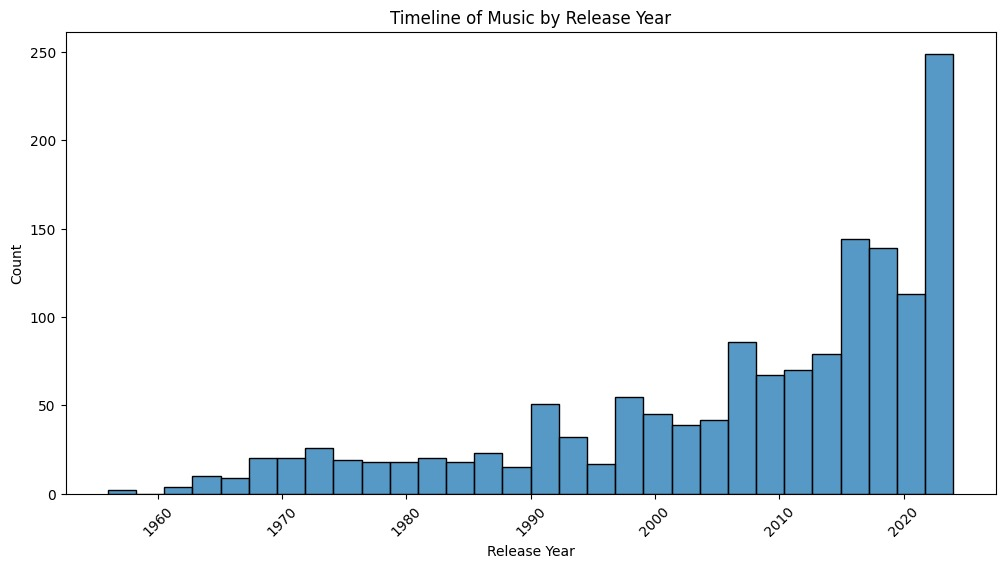
\includegraphics[width=0.5\linewidth]{WhatsApp Image 2024-04-21 at 01.42.27_9751c0c6.jpg}
    \caption{Distribution of Songs}
    \label{fig:Song_Distribution}
\end{figure}
\subsection{Experimental Setting}
We split the dataset for the classifier into training and testing sets for each algorithm using an 80:20 ratio. The training set was used to train the model, while the testing set was used to evaluate its performance. We employed grid search with cross-validation to fine-tune the hyperparameters for each algorithm. \\
\\
For Recommender, the whole dataset was used for training as they all are mostly unsupervised learning, and we can't test how the recommendations are correct, unlike Classifier.
\subsection{Comparison of Results}
\subsubsection{Classifier}
The cross-validation scores for various classifiers are as follows:
\begin{itemize}
    \item Logistic Regression CV: -0.4818295739348371
    \item SGD Classifier CV: 0.21253918495297805
    \item Support Vector Machine CV: 0.29949874686716793
    \item KNN Classifier CV: 0.27962382445141065
    \item Gaussian Naive Bayes CV: 0.42857142857142855
    \item Decision Tree CV: 0.6394984326018809
    \item AdaBoost CV: 0.4868421052631579
    \item XG Boost CV: 0.899749373433584
    \item Random Forest Classifier CV: 0.8564263322884013
    \item Light GBM CV: 0.9015673981191222
    \item MLP Classifier CV: 0.27631578947368424
\end{itemize}
Plots for Classifier:
\begin{figure}[H]
    \centering
    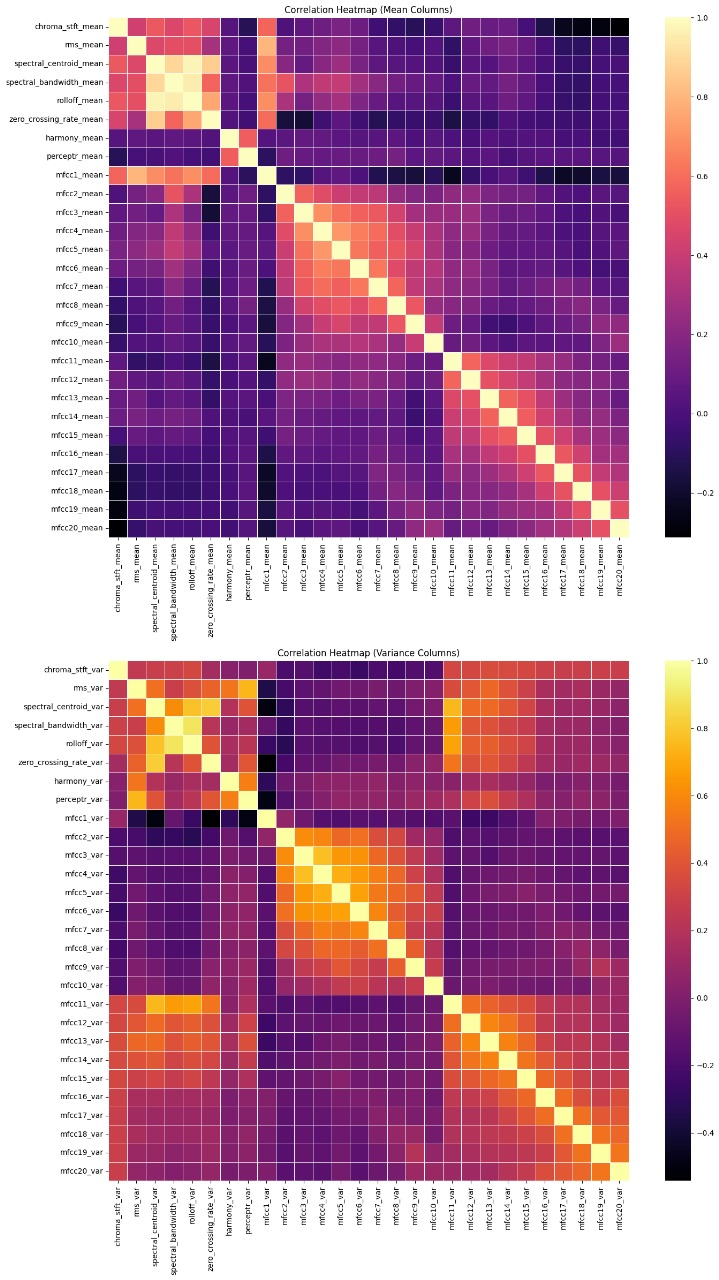
\includegraphics[width=0.5\linewidth]{WhatsApp Image 2024-04-21 at 02.52.30_54356434.jpg}
    \caption{Covariance of the features}
    \label{fig:cov_fea_class}
\end{figure}

\begin{figure}[H]
    \centering
    \begin{subfigure}{0.45\textwidth}
        \centering
        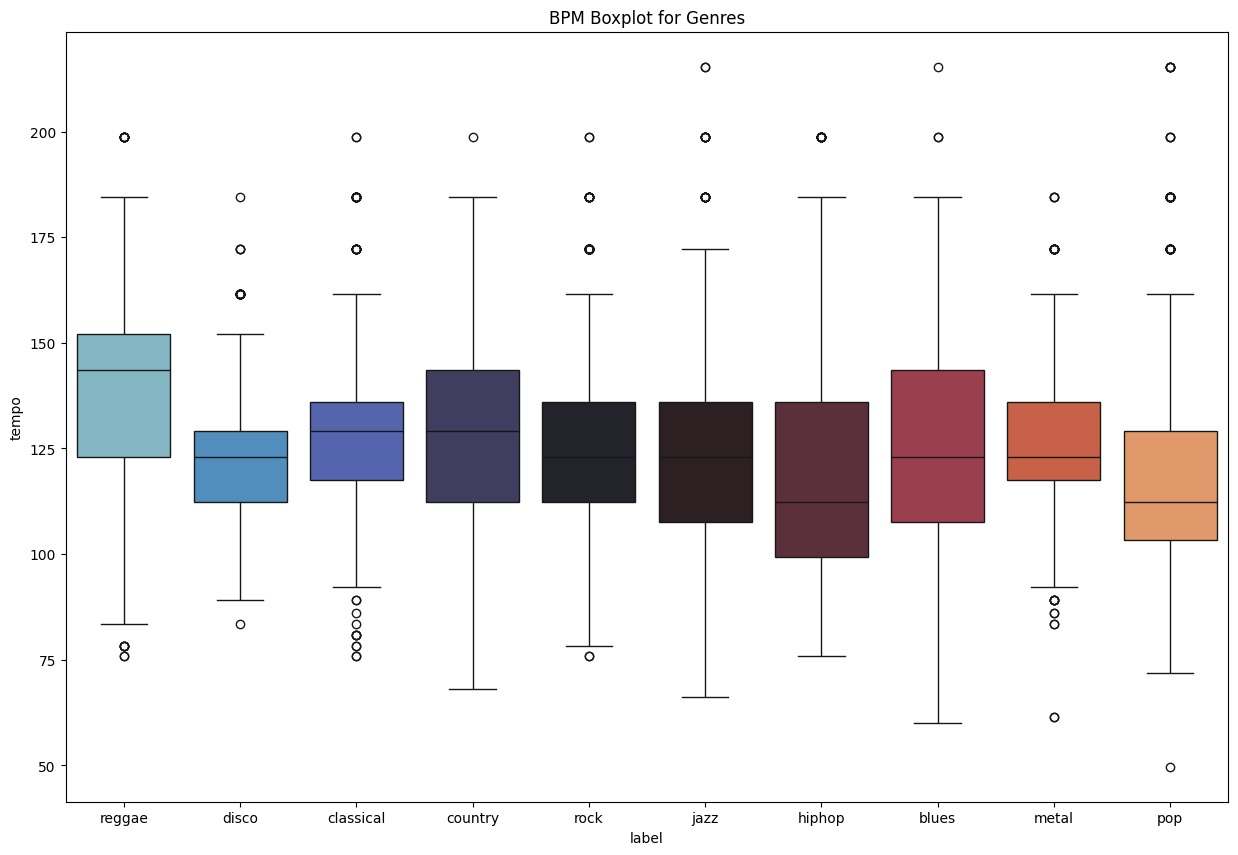
\includegraphics[width=0.5\linewidth]{WhatsApp Image 2024-04-21 at 02.52.50_d518179f.jpg}
        \caption{Boxplots of Data}
        \label{fig:boxplots_class}
    \end{subfigure}
    \hfill
    \begin{subfigure}{0.45\textwidth}
        \centering
        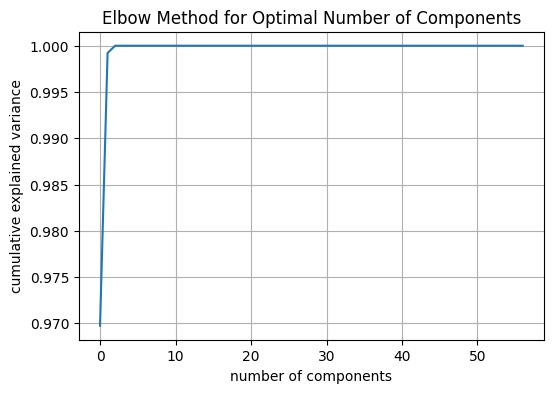
\includegraphics[width=0.5\linewidth]{WhatsApp Image 2024-04-21 at 02.53.05_40714caa.jpg}
        \caption{Better K value for KNN}
        \label{fig:k_knn}
    \end{subfigure}
    \caption{About features of the Data and KNN}
    \label{fig:combined_plots0}
\end{figure}

\begin{figure}[H]
    \centering
    \begin{subfigure}{0.45\textwidth}
        \centering
        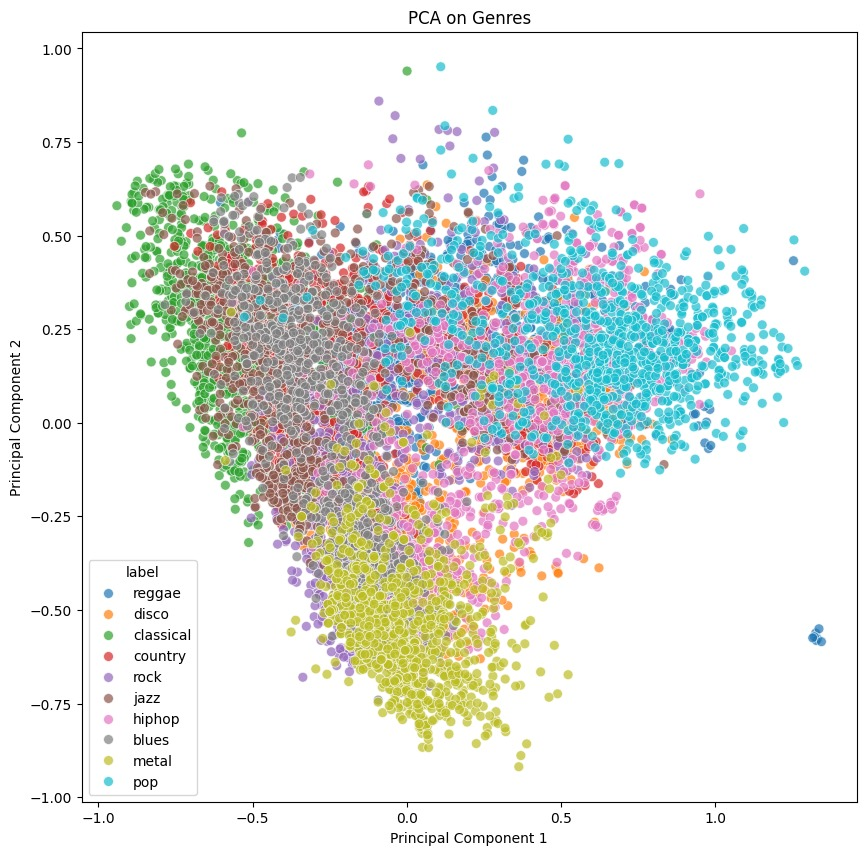
\includegraphics[width=0.5\linewidth]{WhatsApp Image 2024-04-21 at 02.53.22_eae1224c.jpg}
        \caption{PCA on Genres}
        \label{fig:pca_class}
    \end{subfigure}
    \hfill
    \begin{subfigure}{0.45\textwidth}
        \centering
        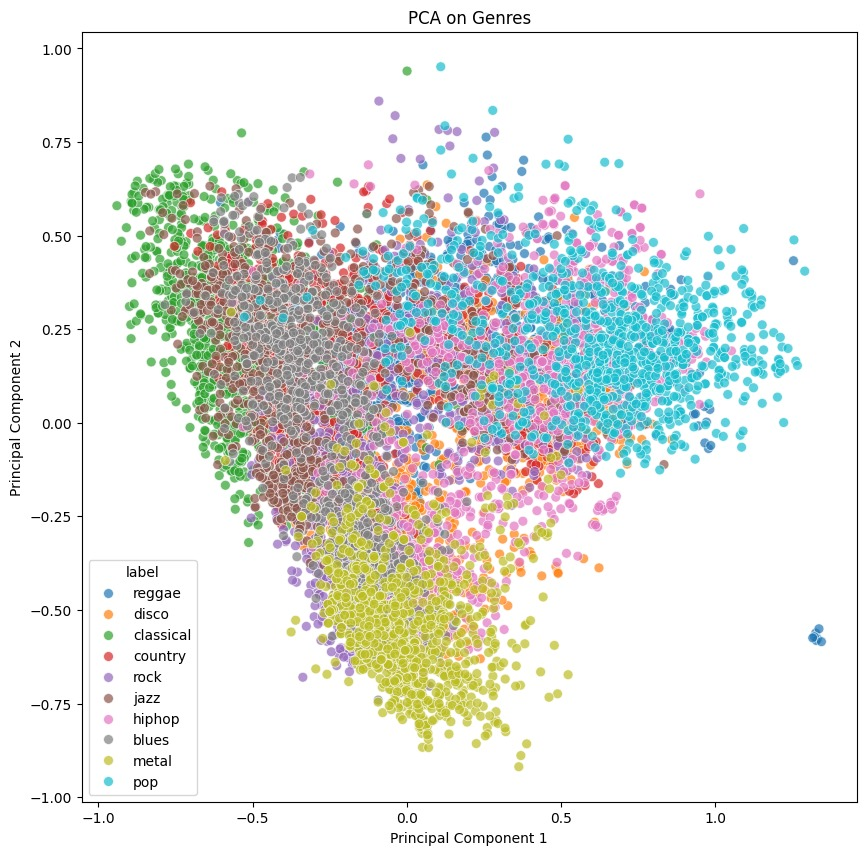
\includegraphics[width=0.5\linewidth]{WhatsApp Image 2024-04-21 at 02.53.22_eae1224cshik.jpg}
        \caption{LDA on Genres}
        \label{fig:lda_class}
    \end{subfigure}
    \caption{PCA and LDA}
    \label{fig:combined_plots0}
\end{figure}
After considering all these factors, we have chosen the Light GBM Classifier as the final classifier for the classifier system.
\subsubsection{Recommender}
These plots are obtained for the data:
\begin{figure}[H]
    \centering
    \begin{subfigure}{0.45\textwidth}
        \centering
        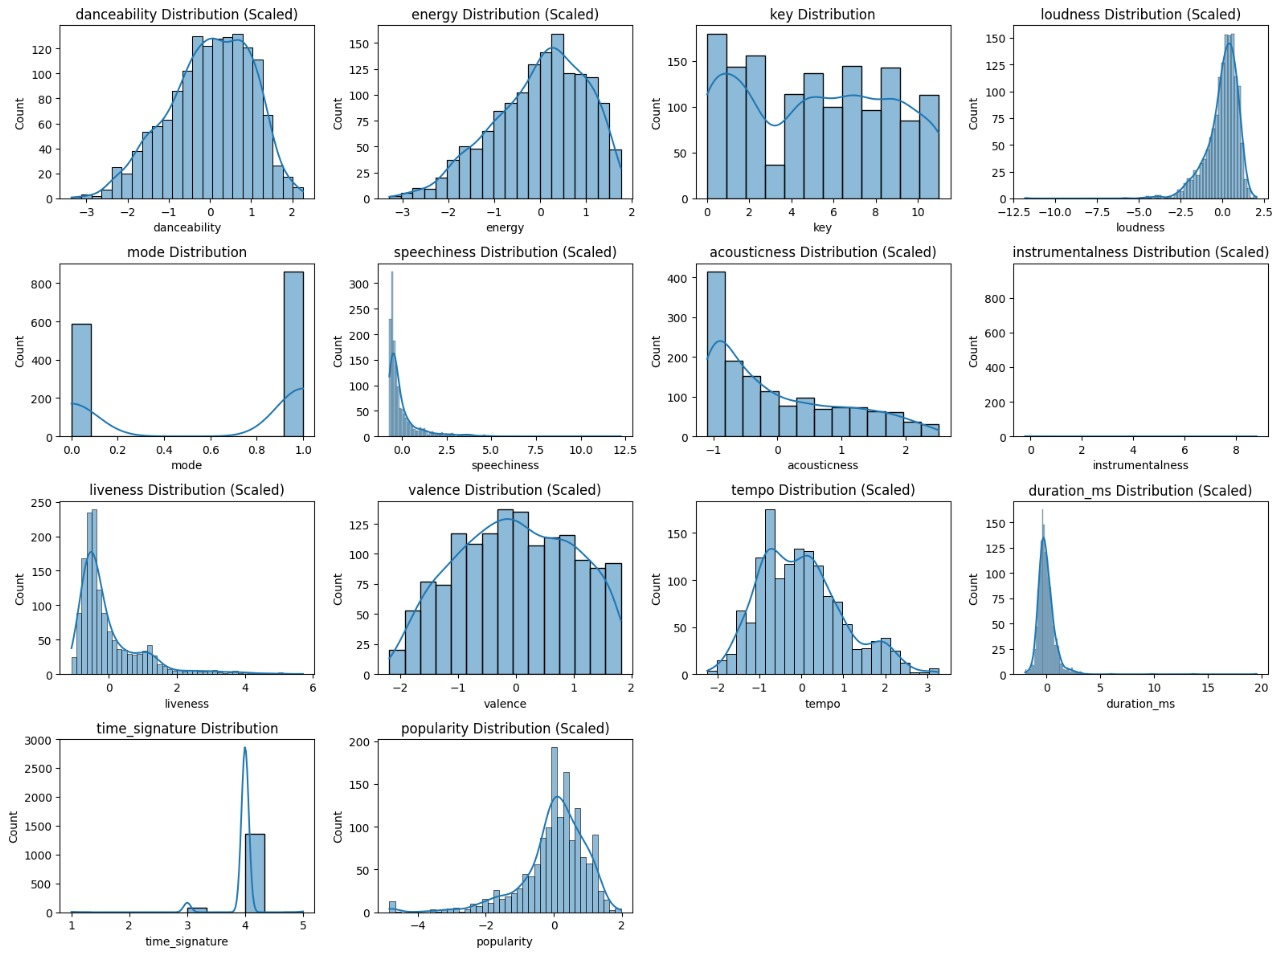
\includegraphics[width=\textwidth]{WhatsApp Image 2024-04-21 at 01.14.08_a32b0b26.jpg}
        \caption{Distribution of features in the dataset.}
        \label{fig:Feature_Distribution of Recommender Data}
    \end{subfigure}
    \hfill
    \begin{subfigure}{0.45\textwidth}
        \centering
        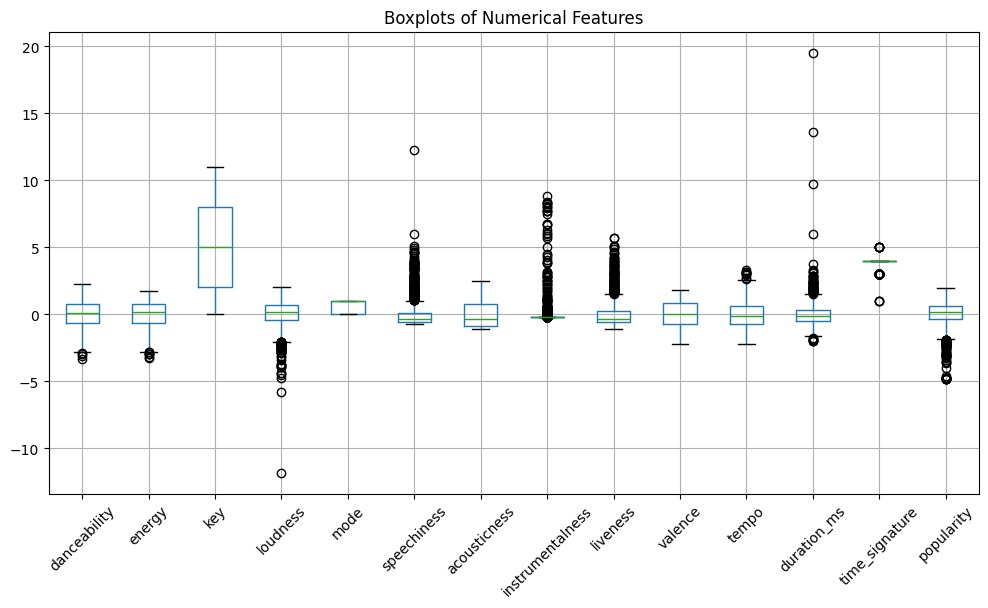
\includegraphics[width=\textwidth]{WhatsApp Image 2024-04-21 at 01.14.32_3b467a5e.jpg}
        \caption{Boxplots of the Features.}
        \label{fig:Boxplots_recmonnd}
    \end{subfigure}
    \caption{About features of the Data}
    \label{fig:combined_plots1}
\end{figure}

These are plots obtained after various approaches used:

\begin{figure}[H]
    \centering
    \begin{subfigure}{0.45\textwidth}
        \centering
        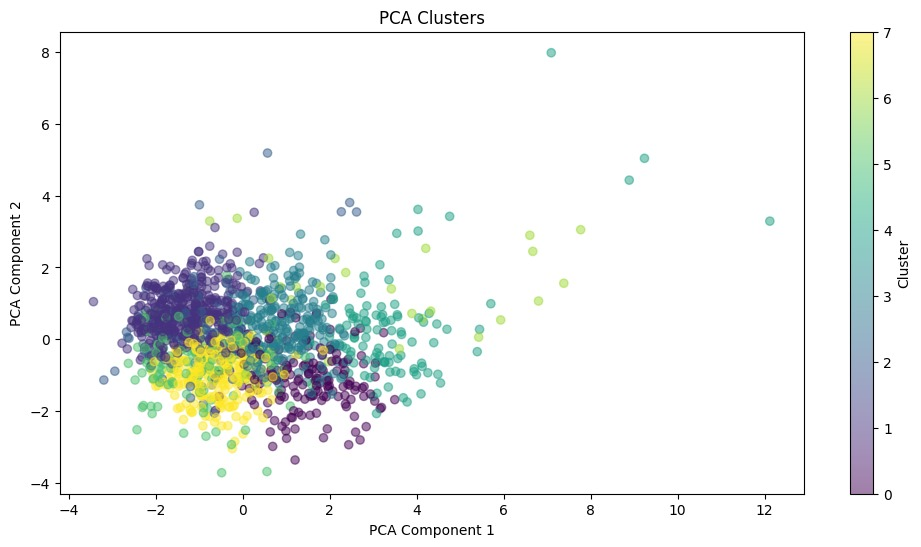
\includegraphics[width=\textwidth]{WhatsApp Image 2024-04-21 at 01.14.38_dc87b777.jpg}
        \caption{PCA plots}
        \label{fig:pca_plots}
    \end{subfigure}
    \hfill
    \begin{subfigure}{0.45\textwidth}
        \centering
        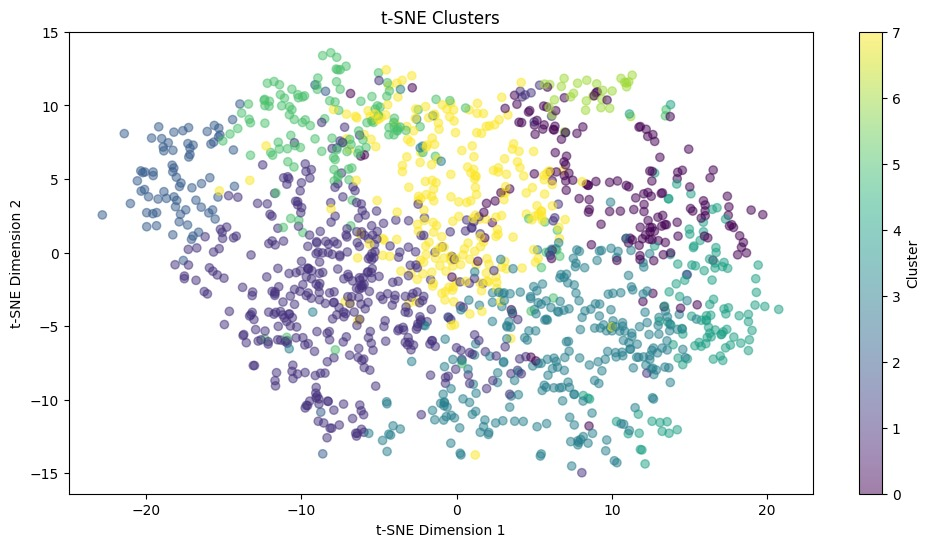
\includegraphics[width=\textwidth]{WhatsApp Image 2024-04-21 at 01.14.43_f7995f40.jpg}
        \caption{t-SNE plots}
        \label{fig:t-sne_plots}
    \end{subfigure}
    \caption{Plots of PCA and t-SNE}
    \label{fig:combined_plots2}
\end{figure}

\begin{figure}[H]
    \centering
    \begin{subfigure}{0.45\textwidth}
        \centering
        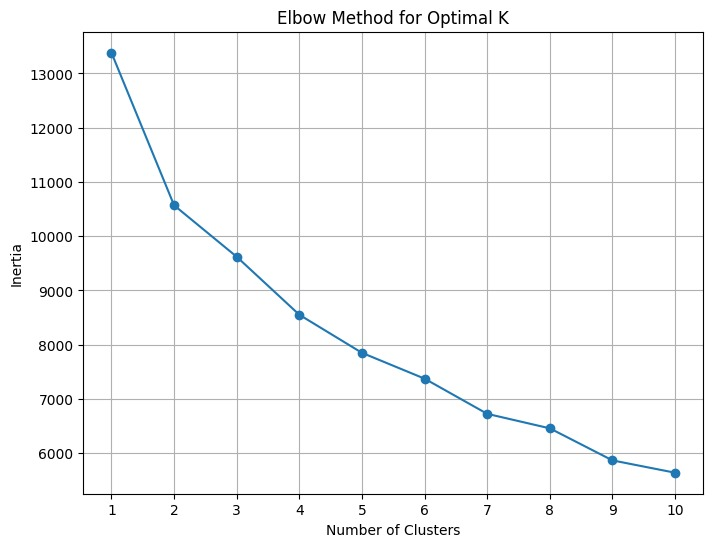
\includegraphics[width=0.5\linewidth]{WhatsApp Image 2024-04-21 at 01.14.47_4e83dc25.jpg}
        \caption{Elbow of K (Kmeans)}
        \label{fig:elbow_k_kmeans}
    \end{subfigure}
    \hfill
    \begin{subfigure}{0.45\textwidth}
        \centering
        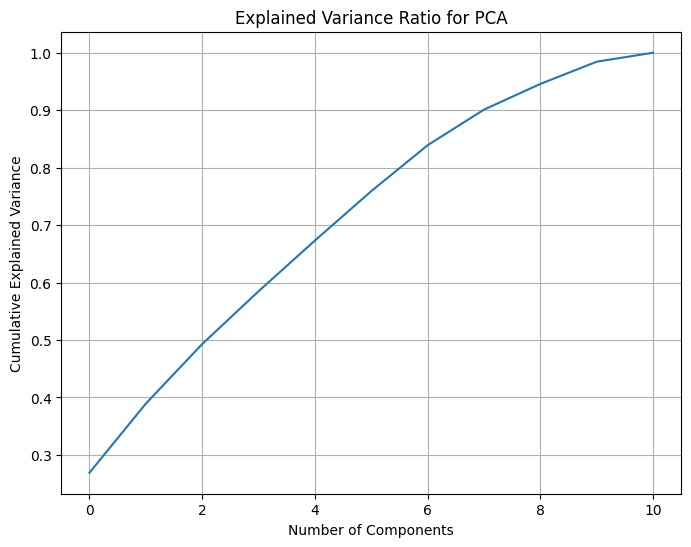
\includegraphics[width=0.5\linewidth]{WhatsApp Image 2024-04-21 at 01.14.54_45ade944.jpg}
        \caption{Explained Variance Ratio}
        \label{fig:exp_var_pca}
        \end{subfigure}
    \caption{Plots of Kmeans and PCA}
    \label{fig:combined_plots3}
\end{figure}
After considering all these factors, our final algorithm is
\paragraph{Recommendation Algorithm}
\subparagraph{General Recommendation Function}
We defined a general recommendation function \texttt{recommend} that utilizes all the computed similarity metrics, KMeans clusters, PCA, and t-SNE to recommend songs based on their similarities.

\subparagraph{Algorithm Description}
The recommendation algorithm works by calculating various similarity scores between the target song and all other songs in the dataset. These scores are then used to identify the most similar songs based on each metric.

\begin{itemize}
    \item \textbf{Similarity Metrics:} For each similarity metric (Cosine Similarity, Euclidean Distance, Manhattan Distance, etc.), we calculate the similarity scores and retrieve the top similar songs.
    
    \item \textbf{KMeans Clustering:} Songs are clustered using KMeans, and a random song from the same cluster as the target song is recommended.
    
    \item \textbf{PCA and t-SNE:} We applied PCA and t-SNE to reduce the dimensionality of our feature space. Then we calculate the distances in the reduced space to recommend songs that are close to the target song in the PCA and t-SNE spaces.
\end{itemize}

\section{Summary}
\label{sec:summary}
The Music Recommendation System project aimed to enhance the user experience on music streaming platforms by introducing a personalized recommendation system. Leveraging machine learning techniques like collaborative and content-based filtering, the system provides tailored music recommendations based on user listening history, preferences, and behavior. The project meticulously explored various machine learning algorithms, including Logistic Regression, SVM, Random Forest, and Light GBM. Evaluations conducted on the GTZAN and Spotify Top Tracks datasets revealed Light GBM as the top-performing classifier, while a hybrid approach incorporating similarity metrics, clustering, PCA, and t-SNE was adopted for the recommender system. The project's findings underscore its potential to revolutionize music discovery and engagement, reflecting a significant enhancement in user satisfaction. Future work could explore further refinements and scalability to accommodate a broader user base and diverse music preferences.

\bibliography{refs}

\newpage

\appendix

\section{Contribution of each member}
\label{sec:contribution}
\begin{enumerate}
\item Sri Ganesh Thota: Worked on Report, Recommender, and Command Line Interface.
\item Rahul Reddy Purmani: Worked on Classifier and Data extraction.
\item Abhijan Theja Katukojwala: Worked on Classifier, Project Page, and Data Collection.
\item Aditya Trivedi Bhargavkumar: Worked on Recommender, Data Collection, and Video Recording.
\item Kaushik Salla: Worked on Classifier, Video Recording, and Data Extraction.
\item Shubham Kumar: Worked on Recommender and Video Recording.
\item Karan Reddy Kanakanala: Worked on Classifier and Project Page.
\end{enumerate}

\end{document}
